\subsection{Equações do Movimento de Atitude da Espaçonave Perseguidora no Referencial Inercial}
\label{sec:atitude_inercial}

A formulação matemática de atitude da espaçonave perseguidora é realizada partir das equações de Euler aplicadas a um corpo rígido.
Essas equações são descritas em torno do centro de massa (\emph{Center of Mass} ou CoM) e expressas no sistema da própria espaçonave.
As equações diferenciais de movimento rotacional assumem a forma \cite{wie2008space}

\begin{equation}
\mathbf{I}\,\dot{\vec{\omega}}
+ \vec{\omega}\times \big(\mathbf{I}\,\vec{\omega}\big)
= \vec{M},
\label{eq:euler_corpo_rigido}
\end{equation}

em que $\mathbf{I}$ é o tensor de inércia em relação ao centro de massa, $\vec{\omega}$ é o vetor de velocidade angular e $\vec{M}$ são os momentos (ou torques) externos aplicados ao corpo.
A equação \eqref{eq:euler_corpo_rigido} é válida somente para a espaçonave perseguidora quando o \gls{mr} não estiver operando, ou seja, travado.

Para um referencial fixo ao corpo, definido pelos eixos principais de inércia $\{x, y, z\}$, as equações rotacionais de Euler que descrevem o movimento de um corpo rígido podem ser expressas como

\begin{equation}
\begin{aligned}
I_x\dot{\omega}_x - (I_y - I_z)\omega_y\omega_z &= M_x, \\[4pt]
I_y\dot{\omega}_y - (I_z - I_x)\omega_z\omega_x &= M_y, \\[4pt]
I_z\dot{\omega}_z - (I_x - I_y)\omega_x\omega_y &= M_z.
\end{aligned}
\end{equation}

Essas três equações diferenciais ordinárias são acopladas e não lineares, além disso, descrevem a evolução das componentes da velocidade angular do corpo rígido.
Em conjunto com as equações cinemáticas correspondentes, elas definem o movimento rotacional de um corpo com três graus de liberdade rotacionais \cite{wie2008space}.

\begin{figure}[ht]
\centering
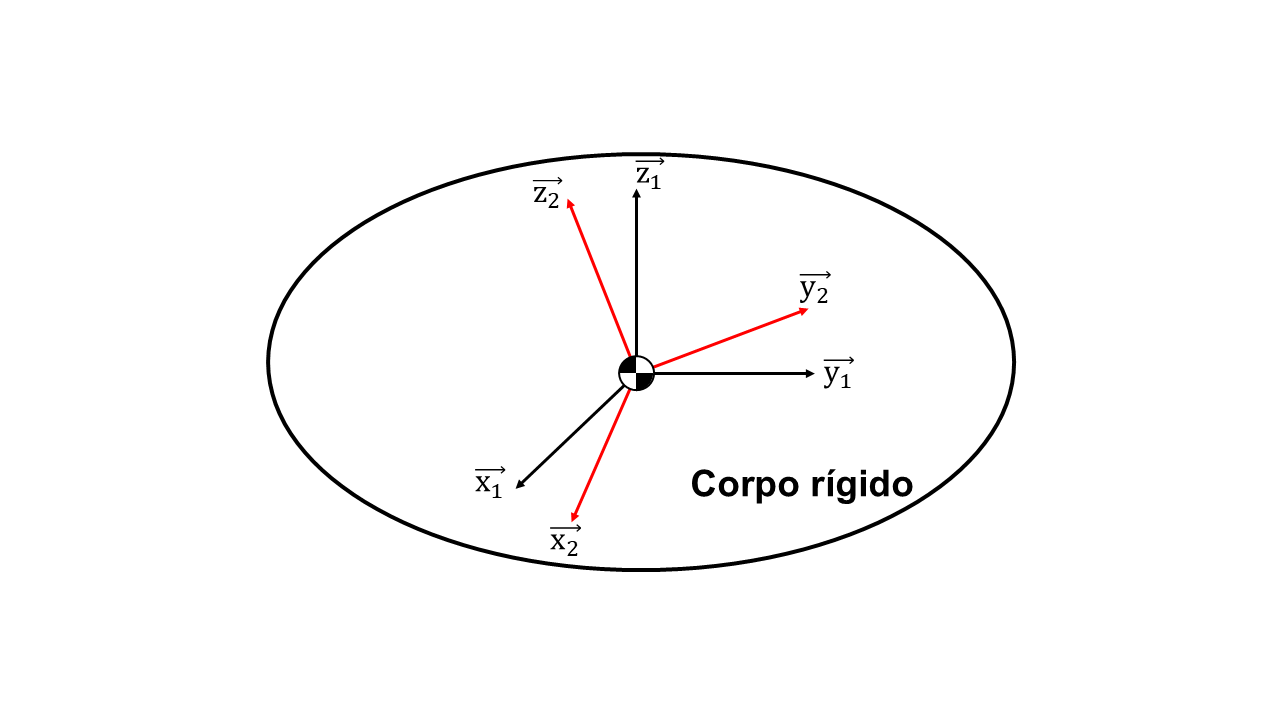
\includegraphics[width=0.9\linewidth]{2 Formulacao matematica/Imagens/Corpo rigido momento.png}
\caption{Corpo rígido com dois referenciais fixos ao corpo. Adaptado de \cite{wie2008space}.}
\label{fig:corpo_rigido_wie_6_3}
\end{figure}

A Figura~\ref{fig:corpo_rigido_wie_6_3} ilustra um corpo rígido, em torno de seu centro de massa.
São mostrados dois sistemas de coordenadas fixos ao corpo, associados aos eixos principais de inércia ${[x, y, z]}$, utilizados para descrever a orientação e o movimento rotacional.
Esses referenciais expressam as componentes da velocidade angular e dos momentos aplicados diretamente no sistema do corpo, conforme as equações de Euler.

Nesse referencial, os eixos ${[x, y, z]}$ estão alinhados com os eixos principais de inércia do corpo, ou seja, aqueles para os quais o tensor de inércia é diagonal.
Portanto, os produtos de inércia são nulos e cada eixo está associado a um momento principal de inércia $[I_x$, $I_y$, $I_z$].
As componentes da velocidade angular $[\omega_x, \omega_y, \omega_z]$ e do momento aplicado $[M_x, M_y, M_z]$ são medidas em relação a esses eixos fixos ao corpo \cite{wie2008space}.

\subsubsection{Tensor de inércia variável}

No caso da espaçonave perseguidora, que possui um \gls{mr} acoplado em sua base, o tensor de inércia não é constante, pois a movimentação dos elos modifica a distribuição de massa, e que pode ser representada por:

\begin{equation}
\mathbf{I}(t) = \mathbf{I}_{base} + \mathbf{I}_{manip}(q(t)),
\label{eq:inercia_total}
\end{equation}

em que $\mathbf{I}_{base}$ é o tensor de inércia associada à base da espaçonave e $\mathbf{I}_{manip}(t)$ é a contribuição variável de inércia do \gls{mr}.
Conforme ocorre a variação temporal de $\mathbf{I}$, o termo $\dot{\mathbf{I}}(t)\omega$ é introduzido na dinâmica do sistema, como visto em \eqref{eq:euler_corpo_rigido}, proposto por \cite{wie2008space}.

A origem do termo adicional se dá a partir da derivada temporal do momento angular, conforme a formulação apresentada em \cite{wie2008space}\fn{Seções 6.2 a 6.4.}.
Considerando o vetor momento angular no sistema do corpo,
$\vec{H} = \mathbf{I}(t)\vec{\omega}$, 
a derivada total no referencial inercial é dada por

\begin{equation}
\frac{d\vec{H}}{dt} = \mathbf{I}(t)\,\dot{\vec{\omega}} + \dot{\mathbf{I}}(t)\,\vec{\omega}.
\label{eq:derivada_momento_angular}
\end{equation}

Substituindo essa expressão na equação geral do momento angular, 
$\vec{M} = \frac{d\vec{H}}{dt} + \vec{\omega}\times\vec{H}$, obtém-se

\begin{equation}
\vec{M} = \mathbf{I}(t)\,\dot{\vec{\omega}} + \dot{\mathbf{I}}(t)\,\vec{\omega} + 
\vec{\omega}\times\big(\mathbf{I}(t)\,\vec{\omega}\big),
\label{eq:euler_inercia_variavel}
\end{equation}

onde o termo $\dot{\mathbf{I}}(t)\vec{\omega}$ representa a contribuição associada 
à variação temporal do tensor de inércia devido à movimentação interna de massas, 
como no caso do manipulador robótico acoplado à base.


% \subsubsection{Dinâmica acoplada com o manipulador}

% Os movimentos do \gls{mr} geram torques que devem ser incluídos na equação dinâmica da atitude, \eqref{eq:euler_corpo_rigido}.
% Deve-se considerar tanto os torques de controle externos quanto os torques internos de reação do MR, dada por:

% \begin{equation}
% \mathbf{I}(t)\,\dot{\vec{\omega}}
% + \vec{\omega}\times \big(\mathbf{I}(t)\,\vec{\omega}\big) 
% = \vec{M}_{controle}
% +\vec{M}_{manip}
% +\mathbf{I}_{manip}
% +\vec \omega_{ferramenta}
% \label{eq:dinamica_acoplada}
% \end{equation}

% onde $\vec{M}_{controle}$ são os torques de controle aplicados à espaçonave e $\vec{M}_{manip}$ são os torques produzidos pelas juntas do MR durante sua movimentação. 